% Created by tikzDevice version 0.12.3.1 on 2022-03-23 09:56:18
% !TEX encoding = UTF-8 Unicode
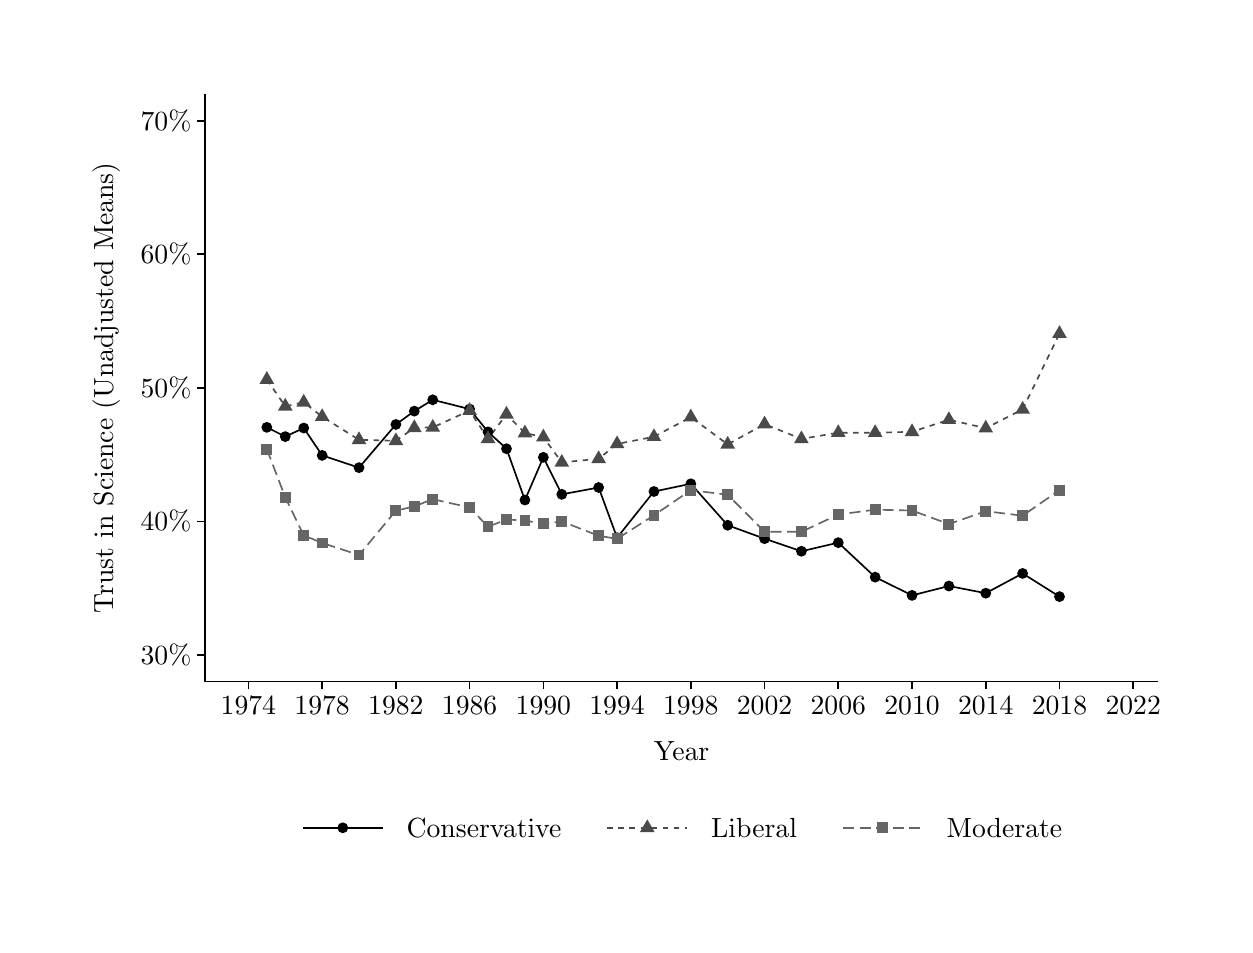
\begin{tikzpicture}[x=1pt,y=1pt]
\definecolor{fillColor}{RGB}{255,255,255}
\path[use as bounding box,fill=fillColor,fill opacity=0.00] (0,0) rectangle (432.48,324.36);
\begin{scope}
\path[clip] (  0.00,  0.00) rectangle (432.48,324.36);
\definecolor{fillColor}{RGB}{255,255,255}

\path[fill=fillColor] ( -0.00,  0.00) rectangle (432.48,324.36);
\end{scope}
\begin{scope}
\path[clip] ( 64.11, 88.07) rectangle (408.48,300.36);
\definecolor{fillColor}{RGB}{255,255,255}

\path[fill=fillColor] ( 64.11, 88.07) rectangle (408.48,300.36);
\definecolor{drawColor}{RGB}{0,0,0}

\path[draw=drawColor,line width= 0.6pt,line join=round] ( 86.42,179.94) --
	( 93.09,176.59) --
	( 99.75,179.69) --
	(106.41,169.80) --
	(119.73,165.37) --
	(133.05,180.97) --
	(139.71,185.80) --
	(146.37,189.89) --
	(159.69,186.54) --
	(166.36,178.29) --
	(173.02,172.22) --
	(179.68,153.66) --
	(186.34,169.10) --
	(193.00,155.72) --
	(206.32,158.20) --
	(212.98,140.06) --
	(226.30,156.75) --
	(239.63,159.54) --
	(252.95,144.55) --
	(266.27,139.71) --
	(279.59,135.16) --
	(292.91,138.27) --
	(306.24,125.81) --
	(319.56,119.22) --
	(332.88,122.60) --
	(346.20,120.01) --
	(359.52,127.15) --
	(372.85,118.77);
\definecolor{drawColor}{gray}{0.29}

\path[draw=drawColor,line width= 0.6pt,dash pattern=on 2pt off 2pt ,line join=round] ( 86.42,197.21) --
	( 93.09,187.53) --
	( 99.75,188.99) --
	(106.41,183.78) --
	(119.73,175.43) --
	(133.05,175.07) --
	(139.71,179.76) --
	(146.37,179.91) --
	(159.69,185.98) --
	(166.36,175.79) --
	(173.02,184.65) --
	(179.68,177.87) --
	(186.34,176.41) --
	(193.00,167.25) --
	(206.32,168.58) --
	(212.98,173.94) --
	(226.30,176.53) --
	(239.63,183.64) --
	(252.95,173.78) --
	(266.27,181.10) --
	(279.59,175.77) --
	(292.91,177.99) --
	(306.24,177.99) --
	(319.56,178.32) --
	(332.88,182.69) --
	(346.20,179.63) --
	(359.52,186.43) --
	(372.85,213.79);
\definecolor{drawColor}{gray}{0.40}

\path[draw=drawColor,line width= 0.6pt,dash pattern=on 4pt off 2pt ,line join=round] ( 86.42,172.08) --
	( 93.09,154.63) --
	( 99.75,140.89) --
	(106.41,138.17) --
	(119.73,133.79) --
	(133.05,149.80) --
	(139.71,151.37) --
	(146.37,153.98) --
	(159.69,150.98) --
	(166.36,144.00) --
	(173.02,146.64) --
	(179.68,146.24) --
	(186.34,145.12) --
	(193.00,145.95) --
	(206.32,140.76) --
	(212.98,139.65) --
	(226.30,148.15) --
	(239.63,157.25) --
	(252.95,155.57) --
	(266.27,142.22) --
	(279.59,142.19) --
	(292.91,148.43) --
	(306.24,150.18) --
	(319.56,149.88) --
	(332.88,144.98) --
	(346.20,149.64) --
	(359.52,148.01) --
	(372.85,157.26);
\definecolor{fillColor}{RGB}{0,0,0}

\path[fill=fillColor] ( 86.42,179.94) circle (  1.96);
\definecolor{fillColor}{gray}{0.29}

\path[fill=fillColor] ( 86.42,200.26) --
	( 89.07,195.68) --
	( 83.78,195.68) --
	cycle;
\definecolor{fillColor}{gray}{0.40}

\path[fill=fillColor] ( 84.46,170.12) --
	( 88.39,170.12) --
	( 88.39,174.04) --
	( 84.46,174.04) --
	cycle;
\definecolor{fillColor}{RGB}{0,0,0}

\path[fill=fillColor] ( 93.09,176.59) circle (  1.96);
\definecolor{fillColor}{gray}{0.29}

\path[fill=fillColor] ( 93.09,190.58) --
	( 95.73,186.00) --
	( 90.44,186.00) --
	cycle;
\definecolor{fillColor}{gray}{0.40}

\path[fill=fillColor] ( 91.12,152.67) --
	( 95.05,152.67) --
	( 95.05,156.59) --
	( 91.12,156.59) --
	cycle;
\definecolor{fillColor}{RGB}{0,0,0}

\path[fill=fillColor] ( 99.75,179.69) circle (  1.96);
\definecolor{fillColor}{gray}{0.29}

\path[fill=fillColor] ( 99.75,192.04) --
	(102.39,187.46) --
	( 97.10,187.46) --
	cycle;
\definecolor{fillColor}{gray}{0.40}

\path[fill=fillColor] ( 97.78,138.93) --
	(101.71,138.93) --
	(101.71,142.85) --
	( 97.78,142.85) --
	cycle;
\definecolor{fillColor}{RGB}{0,0,0}

\path[fill=fillColor] (106.41,169.80) circle (  1.96);
\definecolor{fillColor}{gray}{0.29}

\path[fill=fillColor] (106.41,186.83) --
	(109.05,182.25) --
	(103.76,182.25) --
	cycle;
\definecolor{fillColor}{gray}{0.40}

\path[fill=fillColor] (104.45,136.21) --
	(108.37,136.21) --
	(108.37,140.13) --
	(104.45,140.13) --
	cycle;
\definecolor{fillColor}{RGB}{0,0,0}

\path[fill=fillColor] (119.73,165.37) circle (  1.96);
\definecolor{fillColor}{gray}{0.29}

\path[fill=fillColor] (119.73,178.49) --
	(122.37,173.91) --
	(117.09,173.91) --
	cycle;
\definecolor{fillColor}{gray}{0.40}

\path[fill=fillColor] (117.77,131.83) --
	(121.69,131.83) --
	(121.69,135.75) --
	(117.77,135.75) --
	cycle;
\definecolor{fillColor}{RGB}{0,0,0}

\path[fill=fillColor] (133.05,180.97) circle (  1.96);
\definecolor{fillColor}{gray}{0.29}

\path[fill=fillColor] (133.05,178.12) --
	(135.69,173.54) --
	(130.41,173.54) --
	cycle;
\definecolor{fillColor}{gray}{0.40}

\path[fill=fillColor] (131.09,147.84) --
	(135.01,147.84) --
	(135.01,151.77) --
	(131.09,151.77) --
	cycle;
\definecolor{fillColor}{RGB}{0,0,0}

\path[fill=fillColor] (139.71,185.80) circle (  1.96);
\definecolor{fillColor}{gray}{0.29}

\path[fill=fillColor] (139.71,182.82) --
	(142.35,178.24) --
	(137.07,178.24) --
	cycle;
\definecolor{fillColor}{gray}{0.40}

\path[fill=fillColor] (137.75,149.41) --
	(141.67,149.41) --
	(141.67,153.33) --
	(137.75,153.33) --
	cycle;
\definecolor{fillColor}{RGB}{0,0,0}

\path[fill=fillColor] (146.37,189.89) circle (  1.96);
\definecolor{fillColor}{gray}{0.29}

\path[fill=fillColor] (146.37,182.96) --
	(149.02,178.38) --
	(143.73,178.38) --
	cycle;
\definecolor{fillColor}{gray}{0.40}

\path[fill=fillColor] (144.41,152.02) --
	(148.34,152.02) --
	(148.34,155.94) --
	(144.41,155.94) --
	cycle;
\definecolor{fillColor}{RGB}{0,0,0}

\path[fill=fillColor] (159.69,186.54) circle (  1.96);
\definecolor{fillColor}{gray}{0.29}

\path[fill=fillColor] (159.69,189.03) --
	(162.34,184.45) --
	(157.05,184.45) --
	cycle;
\definecolor{fillColor}{gray}{0.40}

\path[fill=fillColor] (157.73,149.02) --
	(161.66,149.02) --
	(161.66,152.94) --
	(157.73,152.94) --
	cycle;
\definecolor{fillColor}{RGB}{0,0,0}

\path[fill=fillColor] (166.36,178.29) circle (  1.96);
\definecolor{fillColor}{gray}{0.29}

\path[fill=fillColor] (166.36,178.85) --
	(169.00,174.27) --
	(163.71,174.27) --
	cycle;
\definecolor{fillColor}{gray}{0.40}

\path[fill=fillColor] (164.39,142.04) --
	(168.32,142.04) --
	(168.32,145.96) --
	(164.39,145.96) --
	cycle;
\definecolor{fillColor}{RGB}{0,0,0}

\path[fill=fillColor] (173.02,172.22) circle (  1.96);
\definecolor{fillColor}{gray}{0.29}

\path[fill=fillColor] (173.02,187.71) --
	(175.66,183.13) --
	(170.37,183.13) --
	cycle;
\definecolor{fillColor}{gray}{0.40}

\path[fill=fillColor] (171.05,144.68) --
	(174.98,144.68) --
	(174.98,148.60) --
	(171.05,148.60) --
	cycle;
\definecolor{fillColor}{RGB}{0,0,0}

\path[fill=fillColor] (179.68,153.66) circle (  1.96);
\definecolor{fillColor}{gray}{0.29}

\path[fill=fillColor] (179.68,180.92) --
	(182.32,176.34) --
	(177.04,176.34) --
	cycle;
\definecolor{fillColor}{gray}{0.40}

\path[fill=fillColor] (177.72,144.28) --
	(181.64,144.28) --
	(181.64,148.21) --
	(177.72,148.21) --
	cycle;
\definecolor{fillColor}{RGB}{0,0,0}

\path[fill=fillColor] (186.34,169.10) circle (  1.96);
\definecolor{fillColor}{gray}{0.29}

\path[fill=fillColor] (186.34,179.46) --
	(188.98,174.88) --
	(183.70,174.88) --
	cycle;
\definecolor{fillColor}{gray}{0.40}

\path[fill=fillColor] (184.38,143.16) --
	(188.30,143.16) --
	(188.30,147.09) --
	(184.38,147.09) --
	cycle;
\definecolor{fillColor}{RGB}{0,0,0}

\path[fill=fillColor] (193.00,155.72) circle (  1.96);
\definecolor{fillColor}{gray}{0.29}

\path[fill=fillColor] (193.00,170.30) --
	(195.64,165.72) --
	(190.36,165.72) --
	cycle;
\definecolor{fillColor}{gray}{0.40}

\path[fill=fillColor] (191.04,143.99) --
	(194.96,143.99) --
	(194.96,147.91) --
	(191.04,147.91) --
	cycle;
\definecolor{fillColor}{RGB}{0,0,0}

\path[fill=fillColor] (206.32,158.20) circle (  1.96);
\definecolor{fillColor}{gray}{0.29}

\path[fill=fillColor] (206.32,171.63) --
	(208.96,167.05) --
	(203.68,167.05) --
	cycle;
\definecolor{fillColor}{gray}{0.40}

\path[fill=fillColor] (204.36,138.80) --
	(208.28,138.80) --
	(208.28,142.73) --
	(204.36,142.73) --
	cycle;
\definecolor{fillColor}{RGB}{0,0,0}

\path[fill=fillColor] (212.98,140.06) circle (  1.96);
\definecolor{fillColor}{gray}{0.29}

\path[fill=fillColor] (212.98,176.99) --
	(215.63,172.42) --
	(210.34,172.42) --
	cycle;
\definecolor{fillColor}{gray}{0.40}

\path[fill=fillColor] (211.02,137.69) --
	(214.94,137.69) --
	(214.94,141.61) --
	(211.02,141.61) --
	cycle;
\definecolor{fillColor}{RGB}{0,0,0}

\path[fill=fillColor] (226.30,156.75) circle (  1.96);
\definecolor{fillColor}{gray}{0.29}

\path[fill=fillColor] (226.30,179.58) --
	(228.95,175.01) --
	(223.66,175.01) --
	cycle;
\definecolor{fillColor}{gray}{0.40}

\path[fill=fillColor] (224.34,146.18) --
	(228.27,146.18) --
	(228.27,150.11) --
	(224.34,150.11) --
	cycle;
\definecolor{fillColor}{RGB}{0,0,0}

\path[fill=fillColor] (239.63,159.54) circle (  1.96);
\definecolor{fillColor}{gray}{0.29}

\path[fill=fillColor] (239.63,186.69) --
	(242.27,182.11) --
	(236.98,182.11) --
	cycle;
\definecolor{fillColor}{gray}{0.40}

\path[fill=fillColor] (237.66,155.28) --
	(241.59,155.28) --
	(241.59,159.21) --
	(237.66,159.21) --
	cycle;
\definecolor{fillColor}{RGB}{0,0,0}

\path[fill=fillColor] (252.95,144.55) circle (  1.96);
\definecolor{fillColor}{gray}{0.29}

\path[fill=fillColor] (252.95,176.84) --
	(255.59,172.26) --
	(250.31,172.26) --
	cycle;
\definecolor{fillColor}{gray}{0.40}

\path[fill=fillColor] (250.99,153.61) --
	(254.91,153.61) --
	(254.91,157.54) --
	(250.99,157.54) --
	cycle;
\definecolor{fillColor}{RGB}{0,0,0}

\path[fill=fillColor] (266.27,139.71) circle (  1.96);
\definecolor{fillColor}{gray}{0.29}

\path[fill=fillColor] (266.27,184.15) --
	(268.91,179.57) --
	(263.63,179.57) --
	cycle;
\definecolor{fillColor}{gray}{0.40}

\path[fill=fillColor] (264.31,140.26) --
	(268.23,140.26) --
	(268.23,144.18) --
	(264.31,144.18) --
	cycle;
\definecolor{fillColor}{RGB}{0,0,0}

\path[fill=fillColor] (279.59,135.16) circle (  1.96);
\definecolor{fillColor}{gray}{0.29}

\path[fill=fillColor] (279.59,178.82) --
	(282.23,174.24) --
	(276.95,174.24) --
	cycle;
\definecolor{fillColor}{gray}{0.40}

\path[fill=fillColor] (277.63,140.23) --
	(281.55,140.23) --
	(281.55,144.15) --
	(277.63,144.15) --
	cycle;
\definecolor{fillColor}{RGB}{0,0,0}

\path[fill=fillColor] (292.91,138.27) circle (  1.96);
\definecolor{fillColor}{gray}{0.29}

\path[fill=fillColor] (292.91,181.04) --
	(295.56,176.46) --
	(290.27,176.46) --
	cycle;
\definecolor{fillColor}{gray}{0.40}

\path[fill=fillColor] (290.95,146.46) --
	(294.88,146.46) --
	(294.88,150.39) --
	(290.95,150.39) --
	cycle;
\definecolor{fillColor}{RGB}{0,0,0}

\path[fill=fillColor] (306.24,125.81) circle (  1.96);
\definecolor{fillColor}{gray}{0.29}

\path[fill=fillColor] (306.24,181.04) --
	(308.88,176.47) --
	(303.59,176.47) --
	cycle;
\definecolor{fillColor}{gray}{0.40}

\path[fill=fillColor] (304.27,148.21) --
	(308.20,148.21) --
	(308.20,152.14) --
	(304.27,152.14) --
	cycle;
\definecolor{fillColor}{RGB}{0,0,0}

\path[fill=fillColor] (319.56,119.22) circle (  1.96);
\definecolor{fillColor}{gray}{0.29}

\path[fill=fillColor] (319.56,181.37) --
	(322.20,176.79) --
	(316.92,176.79) --
	cycle;
\definecolor{fillColor}{gray}{0.40}

\path[fill=fillColor] (317.60,147.91) --
	(321.52,147.91) --
	(321.52,151.84) --
	(317.60,151.84) --
	cycle;
\definecolor{fillColor}{RGB}{0,0,0}

\path[fill=fillColor] (332.88,122.60) circle (  1.96);
\definecolor{fillColor}{gray}{0.29}

\path[fill=fillColor] (332.88,185.74) --
	(335.52,181.17) --
	(330.24,181.17) --
	cycle;
\definecolor{fillColor}{gray}{0.40}

\path[fill=fillColor] (330.92,143.02) --
	(334.84,143.02) --
	(334.84,146.94) --
	(330.92,146.94) --
	cycle;
\definecolor{fillColor}{RGB}{0,0,0}

\path[fill=fillColor] (346.20,120.01) circle (  1.96);
\definecolor{fillColor}{gray}{0.29}

\path[fill=fillColor] (346.20,182.68) --
	(348.84,178.10) --
	(343.56,178.10) --
	cycle;
\definecolor{fillColor}{gray}{0.40}

\path[fill=fillColor] (344.24,147.67) --
	(348.16,147.67) --
	(348.16,151.60) --
	(344.24,151.60) --
	cycle;
\definecolor{fillColor}{RGB}{0,0,0}

\path[fill=fillColor] (359.52,127.15) circle (  1.96);
\definecolor{fillColor}{gray}{0.29}

\path[fill=fillColor] (359.52,189.48) --
	(362.17,184.91) --
	(356.88,184.91) --
	cycle;
\definecolor{fillColor}{gray}{0.40}

\path[fill=fillColor] (357.56,146.05) --
	(361.49,146.05) --
	(361.49,149.97) --
	(357.56,149.97) --
	cycle;
\definecolor{fillColor}{RGB}{0,0,0}

\path[fill=fillColor] (372.85,118.77) circle (  1.96);
\definecolor{fillColor}{gray}{0.29}

\path[fill=fillColor] (372.85,216.84) --
	(375.49,212.26) --
	(370.20,212.26) --
	cycle;
\definecolor{fillColor}{gray}{0.40}

\path[fill=fillColor] (370.88,155.30) --
	(374.81,155.30) --
	(374.81,159.22) --
	(370.88,159.22) --
	cycle;
\end{scope}
\begin{scope}
\path[clip] (  0.00,  0.00) rectangle (432.48,324.36);
\definecolor{drawColor}{RGB}{0,0,0}

\path[draw=drawColor,line width= 0.6pt,line join=round] ( 64.11, 88.07) --
	( 64.11,300.36);
\end{scope}
\begin{scope}
\path[clip] (  0.00,  0.00) rectangle (432.48,324.36);
\definecolor{drawColor}{RGB}{0,0,0}

\node[text=drawColor,anchor=base east,inner sep=0pt, outer sep=0pt, scale=  1.00] at ( 59.16, 94.27) {30{\%}};

\node[text=drawColor,anchor=base east,inner sep=0pt, outer sep=0pt, scale=  1.00] at ( 59.16,142.52) {40{\%}};

\node[text=drawColor,anchor=base east,inner sep=0pt, outer sep=0pt, scale=  1.00] at ( 59.16,190.77) {50{\%}};

\node[text=drawColor,anchor=base east,inner sep=0pt, outer sep=0pt, scale=  1.00] at ( 59.16,239.02) {60{\%}};

\node[text=drawColor,anchor=base east,inner sep=0pt, outer sep=0pt, scale=  1.00] at ( 59.16,287.27) {70{\%}};
\end{scope}
\begin{scope}
\path[clip] (  0.00,  0.00) rectangle (432.48,324.36);
\definecolor{drawColor}{RGB}{0,0,0}

\path[draw=drawColor,line width= 0.6pt,line join=round] ( 61.36, 97.72) --
	( 64.11, 97.72);

\path[draw=drawColor,line width= 0.6pt,line join=round] ( 61.36,145.96) --
	( 64.11,145.96);

\path[draw=drawColor,line width= 0.6pt,line join=round] ( 61.36,194.21) --
	( 64.11,194.21);

\path[draw=drawColor,line width= 0.6pt,line join=round] ( 61.36,242.46) --
	( 64.11,242.46);

\path[draw=drawColor,line width= 0.6pt,line join=round] ( 61.36,290.71) --
	( 64.11,290.71);
\end{scope}
\begin{scope}
\path[clip] (  0.00,  0.00) rectangle (432.48,324.36);
\definecolor{drawColor}{RGB}{0,0,0}

\path[draw=drawColor,line width= 0.6pt,line join=round] ( 64.11, 88.07) --
	(408.48, 88.07);
\end{scope}
\begin{scope}
\path[clip] (  0.00,  0.00) rectangle (432.48,324.36);
\definecolor{drawColor}{RGB}{0,0,0}

\path[draw=drawColor,line width= 0.6pt,line join=round] ( 79.76, 85.32) --
	( 79.76, 88.07);

\path[draw=drawColor,line width= 0.6pt,line join=round] (106.41, 85.32) --
	(106.41, 88.07);

\path[draw=drawColor,line width= 0.6pt,line join=round] (133.05, 85.32) --
	(133.05, 88.07);

\path[draw=drawColor,line width= 0.6pt,line join=round] (159.69, 85.32) --
	(159.69, 88.07);

\path[draw=drawColor,line width= 0.6pt,line join=round] (186.34, 85.32) --
	(186.34, 88.07);

\path[draw=drawColor,line width= 0.6pt,line join=round] (212.98, 85.32) --
	(212.98, 88.07);

\path[draw=drawColor,line width= 0.6pt,line join=round] (239.63, 85.32) --
	(239.63, 88.07);

\path[draw=drawColor,line width= 0.6pt,line join=round] (266.27, 85.32) --
	(266.27, 88.07);

\path[draw=drawColor,line width= 0.6pt,line join=round] (292.91, 85.32) --
	(292.91, 88.07);

\path[draw=drawColor,line width= 0.6pt,line join=round] (319.56, 85.32) --
	(319.56, 88.07);

\path[draw=drawColor,line width= 0.6pt,line join=round] (346.20, 85.32) --
	(346.20, 88.07);

\path[draw=drawColor,line width= 0.6pt,line join=round] (372.85, 85.32) --
	(372.85, 88.07);

\path[draw=drawColor,line width= 0.6pt,line join=round] (399.49, 85.32) --
	(399.49, 88.07);
\end{scope}
\begin{scope}
\path[clip] (  0.00,  0.00) rectangle (432.48,324.36);
\definecolor{drawColor}{RGB}{0,0,0}

\node[text=drawColor,anchor=base,inner sep=0pt, outer sep=0pt, scale=  1.00] at ( 79.76, 76.23) {1974};

\node[text=drawColor,anchor=base,inner sep=0pt, outer sep=0pt, scale=  1.00] at (106.41, 76.23) {1978};

\node[text=drawColor,anchor=base,inner sep=0pt, outer sep=0pt, scale=  1.00] at (133.05, 76.23) {1982};

\node[text=drawColor,anchor=base,inner sep=0pt, outer sep=0pt, scale=  1.00] at (159.69, 76.23) {1986};

\node[text=drawColor,anchor=base,inner sep=0pt, outer sep=0pt, scale=  1.00] at (186.34, 76.23) {1990};

\node[text=drawColor,anchor=base,inner sep=0pt, outer sep=0pt, scale=  1.00] at (212.98, 76.23) {1994};

\node[text=drawColor,anchor=base,inner sep=0pt, outer sep=0pt, scale=  1.00] at (239.63, 76.23) {1998};

\node[text=drawColor,anchor=base,inner sep=0pt, outer sep=0pt, scale=  1.00] at (266.27, 76.23) {2002};

\node[text=drawColor,anchor=base,inner sep=0pt, outer sep=0pt, scale=  1.00] at (292.91, 76.23) {2006};

\node[text=drawColor,anchor=base,inner sep=0pt, outer sep=0pt, scale=  1.00] at (319.56, 76.23) {2010};

\node[text=drawColor,anchor=base,inner sep=0pt, outer sep=0pt, scale=  1.00] at (346.20, 76.23) {2014};

\node[text=drawColor,anchor=base,inner sep=0pt, outer sep=0pt, scale=  1.00] at (372.85, 76.23) {2018};

\node[text=drawColor,anchor=base,inner sep=0pt, outer sep=0pt, scale=  1.00] at (399.49, 76.23) {2022};
\end{scope}
\begin{scope}
\path[clip] (  0.00,  0.00) rectangle (432.48,324.36);
\definecolor{drawColor}{RGB}{0,0,0}

\node[text=drawColor,anchor=base,inner sep=0pt, outer sep=0pt, scale=  1.00] at (236.30, 59.40) {Year};
\end{scope}
\begin{scope}
\path[clip] (  0.00,  0.00) rectangle (432.48,324.36);
\definecolor{drawColor}{RGB}{0,0,0}

\node[text=drawColor,rotate= 90.00,anchor=base,inner sep=0pt, outer sep=0pt, scale=  1.00] at ( 30.89,194.21) {Trust in Science (Unadjusted Means)};
\end{scope}
\begin{scope}
\path[clip] (  0.00,  0.00) rectangle (432.48,324.36);

\path[] ( 86.80, 24.00) rectangle (385.79, 46.45);
\end{scope}
\begin{scope}
\path[clip] (  0.00,  0.00) rectangle (432.48,324.36);

\path[] ( 95.80, 28.00) rectangle (131.94, 42.45);
\end{scope}
\begin{scope}
\path[clip] (  0.00,  0.00) rectangle (432.48,324.36);
\definecolor{drawColor}{RGB}{0,0,0}

\path[draw=drawColor,line width= 0.6pt,line join=round] ( 99.42, 35.23) -- (128.33, 35.23);
\end{scope}
\begin{scope}
\path[clip] (  0.00,  0.00) rectangle (432.48,324.36);
\definecolor{fillColor}{RGB}{0,0,0}

\path[fill=fillColor] (113.87, 35.23) circle (  1.96);
\end{scope}
\begin{scope}
\path[clip] (  0.00,  0.00) rectangle (432.48,324.36);

\path[] (205.84, 28.00) rectangle (241.98, 42.45);
\end{scope}
\begin{scope}
\path[clip] (  0.00,  0.00) rectangle (432.48,324.36);
\definecolor{drawColor}{gray}{0.29}

\path[draw=drawColor,line width= 0.6pt,dash pattern=on 2pt off 2pt ,line join=round] (209.46, 35.23) -- (238.36, 35.23);
\end{scope}
\begin{scope}
\path[clip] (  0.00,  0.00) rectangle (432.48,324.36);
\definecolor{fillColor}{gray}{0.29}

\path[fill=fillColor] (223.91, 38.28) --
	(226.55, 33.70) --
	(221.27, 33.70) --
	cycle;
\end{scope}
\begin{scope}
\path[clip] (  0.00,  0.00) rectangle (432.48,324.36);

\path[] (290.97, 28.00) rectangle (327.10, 42.45);
\end{scope}
\begin{scope}
\path[clip] (  0.00,  0.00) rectangle (432.48,324.36);
\definecolor{drawColor}{gray}{0.40}

\path[draw=drawColor,line width= 0.6pt,dash pattern=on 4pt off 2pt ,line join=round] (294.58, 35.23) -- (323.49, 35.23);
\end{scope}
\begin{scope}
\path[clip] (  0.00,  0.00) rectangle (432.48,324.36);
\definecolor{fillColor}{gray}{0.40}

\path[fill=fillColor] (307.07, 33.26) --
	(311.00, 33.26) --
	(311.00, 37.19) --
	(307.07, 37.19) --
	cycle;
\end{scope}
\begin{scope}
\path[clip] (  0.00,  0.00) rectangle (432.48,324.36);
\definecolor{drawColor}{RGB}{0,0,0}

\node[text=drawColor,anchor=base west,inner sep=0pt, outer sep=0pt, scale=  1.00] at (136.94, 31.78) {Conservative};
\end{scope}
\begin{scope}
\path[clip] (  0.00,  0.00) rectangle (432.48,324.36);
\definecolor{drawColor}{RGB}{0,0,0}

\node[text=drawColor,anchor=base west,inner sep=0pt, outer sep=0pt, scale=  1.00] at (246.98, 31.78) {Liberal};
\end{scope}
\begin{scope}
\path[clip] (  0.00,  0.00) rectangle (432.48,324.36);
\definecolor{drawColor}{RGB}{0,0,0}

\node[text=drawColor,anchor=base west,inner sep=0pt, outer sep=0pt, scale=  1.00] at (332.10, 31.78) {Moderate};
\end{scope}
\end{tikzpicture}
